\documentclass[twoside, letterpaper, 12pt]{report}
\usepackage{orthodoxservicebook}

\title{The Sunday Reader's Service of the \\ \textsc{Typica} \\ 2020 July 12}
\titlepic{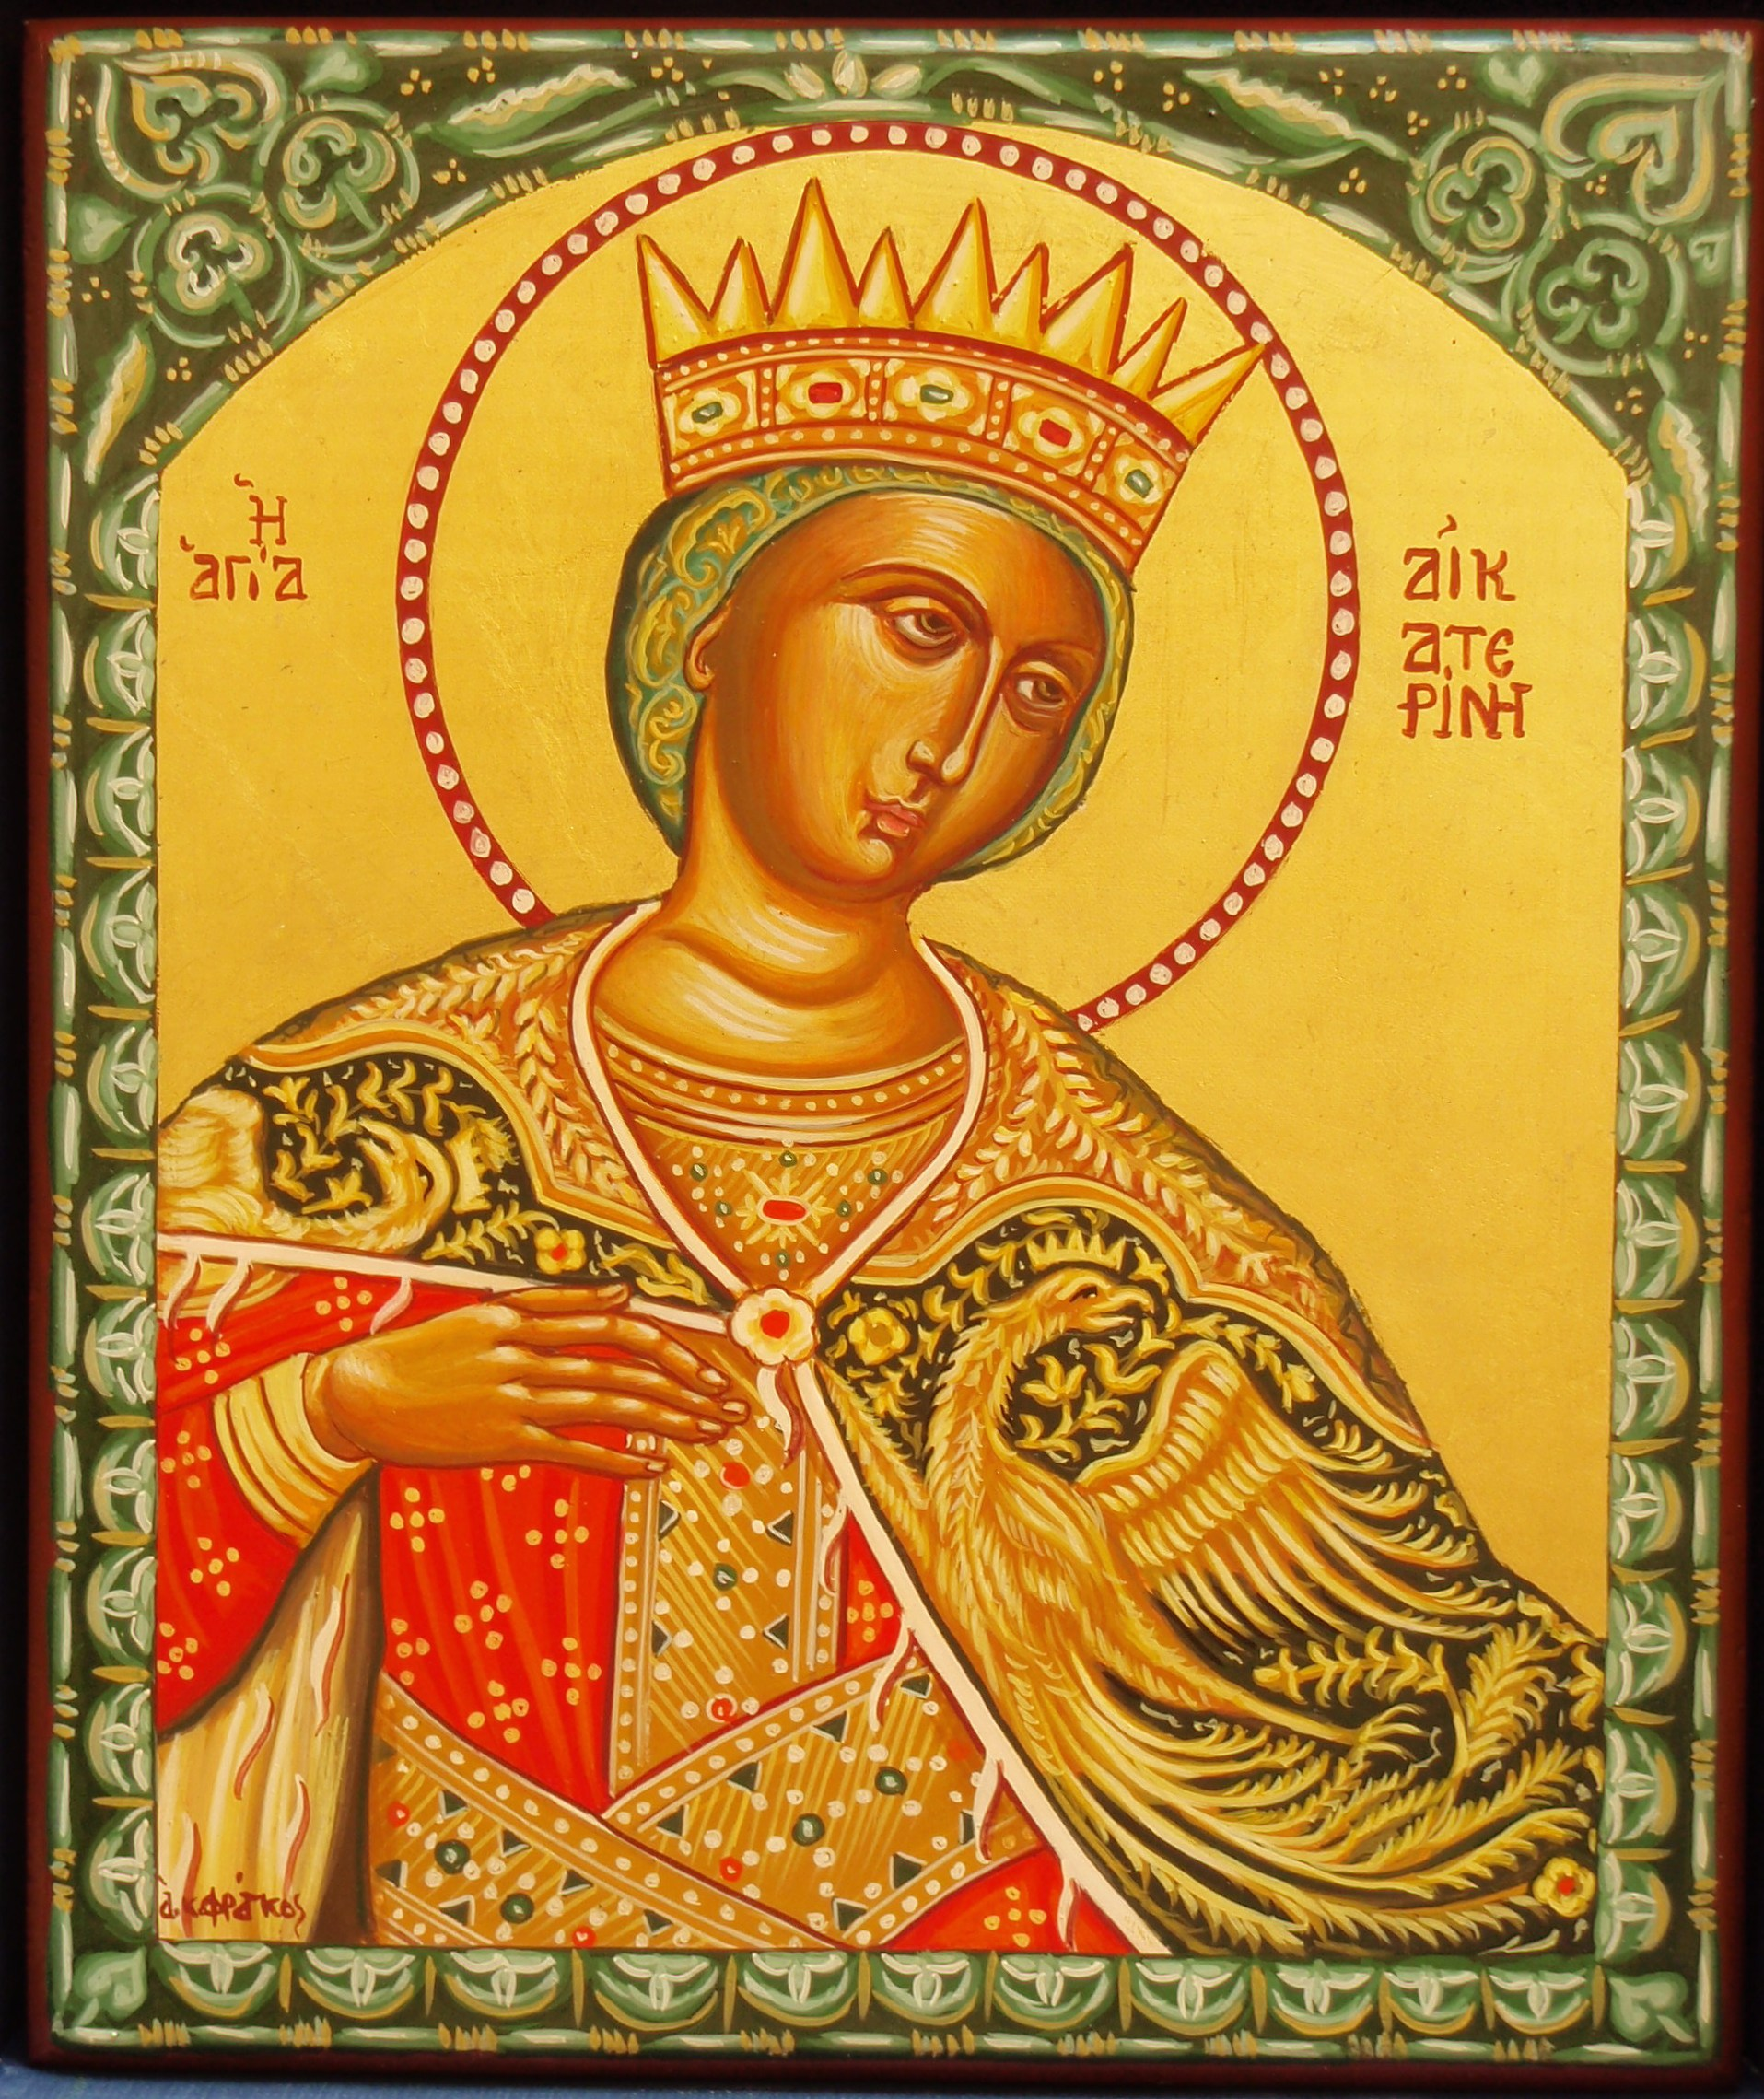
\includegraphics[width=0.5\textwidth]{Katherine1.jpg}}
\date{}
\author{}

\begin{document}
\maketitle
\pagestyle{empty} % Don't show page numbers
\instruction{This page intentionally left blank}
\cleardoublepage
\pagestyle{plain}
\setcounter{page}{1} % Set the page counter to 1 on the first real page
\chapter*{Service of Typica on Sunday, June 12}
\instruction{The Great Feast of Pentecost\\
Fiftieth Day After Pascha}

\readerline{\throughtheprayers{}}
\choralresponse{./Z-Responses/Obikhod/Amen.ly}

\trisagionNeedsAmen[reader]

\choralresponse{./Z-Responses/Obikhod/Amen.ly}


\centeredsection{The First Antiphon}
\lilypondfile{./Liturgy/B-FirstAntiphon/BlessTheLord_Greek-Music.ly}

\centeredsection{The Second Antiphon}
\lilypondfile{./Liturgy/C-SecondAntiphon/PraiseTheLord_Greek-Music.ly}

\centeredsection{The Third Antiphon}
\lilypondfile{./Liturgy/D-ThirdAntiphon/Beatitudes_Moscow-Music.ly}

\centeredsection{The Epistle}

\instruction{Both of the New Testament lessons are read
without liturgical introduction or conclusion.
The readers start with “The Reading from…” and proceeds}

\paragraph{The Reading from the Epistle of St. Paul to the Romans. (10:1-10)}\mbox{}\\

\begin{maybetwocolumns}
  Brethren, my heart’s desire and prayer to God for Israel is that it may be saved. I bear them
  witness that they have a zeal for God, but it is not enlightened. For, being ignorant of the
  righteousness that comes from God, and seeking to establish their own, they did not submit to
  God’s righteousness. For Christ is the end of the law, that everyone who has faith may be justified.
  Moses writes that the man who practices the righteousness which is based on the law shall live by
  it. But the righteousness based on faith says: Do not say in your heart, “Who will ascend into
  Heaven?” (that is, to bring Christ down) or “Who will descend into the abyss?” (that is, to bring
  Christ up from the dead). But what does it say? The word is near you, on your lips and in your
  heart (that is, the word of faith which we preach); because, if you confess with your lips that Jesus
  is Lord and believe in your heart that God raised Him from the dead, you will be saved. For man
  believes with his heart and so is justified, and he confesses with his lips and so is saved.
\end{maybetwocolumns}

\centeredsection{The Gospel}

\instruction{Both of the New Testament lessons are read
without liturgical introduction or conclusion.
The readers start with “The Reading from…” and proceeds}

\paragraph{The Reading from the Holy Gospel according to St. Matthew. (8:28-9:1)}\mbox{}\\

\begin{maybetwocolumns}
  At that time, when Jesus came to the country of the Gergesenes, two demoniacs met Him,
  coming out of the tombs, so fierce that no one could pass that way. And behold, they cried out,
  “What have we to do to Thee, O Son of God? Art Thou come here to torment us before the time?”
  Now a herd of many swine was feeding at some distance from them. And the demons begged Him,
  “If Thou castest us out, send us away into the herd of swine.” And He said to them, “Go.” So they
  came out and went into the swine; and behold, the whole herd rushed down the steep bank into the
  sea, and perished in the waters. The herdsmen fled, and going into the city they told everything,
  and what had happened to the demoniacs. And behold, all the city came out to meet Jesus; and
  when they saw Him, they begged Him to leave their neighborhood. And getting into a boat He
  crossed over and came to His own city.
\end{maybetwocolumns}

\centeredsection{Troparia Before the Creed}
\instruction{Plain reading}
\begin{reader}
\item[Reader 1:] The heavenly choir singeth thy praises, saying:
  Holy, holy, holy, Lord of Sabaoth; heaven and earth are full of Thy glory.

\item[Reader 2:] \emph{Come unto him, and be enlightened,
               and your faces shall not be ashamed.}
  The heavenly choir singeth thy praises, saying:
  Holy, holy, holy, Lord of Sabaoth; heaven and earth are full of Thy glory.

\item[Reader 1:] \emph{\glory}
  The choir of the holy angels and archangels,
  with all the powers of heaven, singeth thy praises, saying:
  Holy, holy, holy, Lord of Sabaoth; heaven and earth are full of Thy glory.

\item[Reader 2:]\emph{\nowandever}
\end{reader}

\centeredsection{The Creed}
\input{Common/TheCreed.txt}


\centeredsection{Prayer of Forgiveness}
\readerline{Forgive, remit, pardon, O God, our sins,
  both voluntary and involuntary, in deed and in word, in knowledge or in ignorance,
  committed by night or by day, in mind and in thought.
  Forgive us them all, for thou art good and lovest mankind.
}

\centeredsection{The Lord’s Prayer}
\input{Common/LordsPrayer.txt}

\readerline{Through the prayers of our holy fathers, Lord Jesus Christ our God, have mercy on us.}
\choralresponse{./Z-Responses/Obikhod/Amen.ly}

\centeredsection{Kontakia for Normal Sudays}
\lilypondfile{./Liturgy/H-Kontakion/OProtectionOfChristians_Tone2ByzChant-Music.ly}

\readerline{\lhmForty}

\readerline{
  O Christ our God, Who art worshipped and glorified at all times at every hour both in
  heaven and on earth; Who art long-suffering and plenteous in mercy and compassion; Who lovest
  the just man and showest mercy upon the sinner; and Who callest all men to repentance through 
  the promise of blessings to come; receive, O Lord, at this very hour our supplications, and direct
  our lives in the way of Thy commandments: sanctify our souls, purify our bodies, set our minds
  aright, cleanse our thoughts; deliver us from all affliction, trouble, and distress; compass us about
  with Thy holy angels, that, guided and guarded by them, we may attain unto the unity of the Faith,
  and to the knowledge of Thine unapproachable glory; for Thou art blessed unto ages of ages. Amen.
}

\begin{reader}
  \item \lhmThree{}\\\emph{\gne{}}
  \item \morehonorablethanthetherubim{}
  \item \throughtheprayers{}
\end{reader}

\begin{maybetwocolumns}
\choralresponse{./Z-Responses/Obikhod/Amen.ly}

\readerline{\blessedbethename{}\thrice{}}

\centeredsection{Psalm 33}
\input{./Psalms/Psalm033-unknowntrans.txt}

\end{maybetwocolumns}

\peopleline{\gne}


\centeredsection{A Homily}
\begin{maybetwocolumns}
\instruction{Becoming Our True Selves Through Faith in Christ:\\
  Homily for the Fifth Sunday After Pentecost and the Fifth Sunday of Matthew in the Orthodox Church\\
}

The many challenges that we face today should open our eyes to uncomfortable truths about what it
means to be a human person in the world as we know it.  The pandemic shows that we remain subject to
death and disease in ways that no one can fully control.  Our social and economic crises reveal that
no nation or culture embodies the fulfillment of the collective life of humankind.  Such struggles
display not only how weak we are before large matters beyond our control, but also our captivity to
our own passions.  Self-centeredness, fear, resentment, and even hatred easily fill our hearts as
ways of coping with problems that challenge our proud illusions.  Instead of simply accepting what
our disordered desires reveal about us and embracing the truth for our humility, we typically prefer
the distraction of blaming others or at least of thinking of something else that turns our attention
away from reality.

If we think we have remarkable problems today, consider for a moment the plight of the
demon-possessed men in our gospel reading.  The Savior did not require them to become Jews, obey a
law, or do anything else.  He simply set them free from slavery to evil and restored them to a
recognizably human existence. The Fathers of the Church see their demon-possession as symbolic of
the state of our ancestors, the Gentiles who worshiped idols and false gods.  As St. Paul wrote to
the Romans:  “Christ is the end of the law for righteousness to everyone who believes.”  At the very
heart of our faith is not a requirement to belong to any nation, class, or race, but instead the
outrageous mercy of the Lord Who restores us to the dignity of those created in the divine image and
likeness. The good news of the Gospel is that the Son of God became a human being for the salvation
of all people, including those as lowly and miserable as demon-possessed Gentiles living in a tomb
and scaring everyone away.

Just as Christ took the initiative to deliver them, He has done the same with everyone.  He has
become one of us, taking upon Himself the consequences of all human corruption and sin to the point
of death, burial, and descent into Hades so that He could conquer them all in His glorious third-day
resurrection.  He has ascended into heaven with full, complete glorified humanity and sent the Holy
Spirit to empower His Body, the Church, of which we are living members.  He abides within our hearts
by the Holy Spirit, casting out our demons, forgiving our sins, and enabling us to share in His
eternal life even now.

As St. Paul teaches, we must confess the Lord Jesus Christ with our mouths and believe in our hearts
that God has raised him from the dead; if we do so, we will be saved.  “For with the heart one
believes unto righteousness and with the mouth confession is made unto salvation.”   No, St. Paul is
not giving us magic words which we say once in order to guarantee a spot in heaven.  He is not
giving us a new religious legalism that somehow earns salvation.  Instead, He reminds us that we
must commend our entire life to Christ our God.  If we trust in Him, we will offer our words, deeds,
and thoughts to embody the healing that He has brought to the world.  He calls and enables us to
become as transformed by the divine mercy as were the demon-possessed men who became powerful living
examples of His salvation.

When those men were set free from the complete control of demons, that was only the beginning of
their lives in Christ.  Even though their deliverance was quite dramatic, it was only a beginning
and they surely had to press on from there to resist temptation, to grow in holiness, and to learn
to love and serve the Savior in their neighbors.  The very same thing is true of us.  The healing of
our souls is a process, an ongoing journey of sharing more fully in the new life that our Savior has
brought to the world.  Challenges large and small require us to confess Christ faithfully each day
of our lives in what we say, think, and do.

To believe in and confess Christ is never something that we should think we have accomplished or
fulfilled.  To be perfect as our Father in heaven is perfect is an eternal goal.  To become a
partaker of the divine nature is truly an infinite undertaking.  Believing in and confessing Christ
requires that we share in His life without reservation such that His restoration of the human person
in the divine likeness shines brilliantly in us.  Only then we will be able to stay with St. Paul,
“It is no longer I who live, but Christ Who lives in me.”    That change will not happen in an
instant, but will be as profoundly transformative as what happened to the demon-possessed men who
regained their true selves by encountering the Savior.  That is what will happen with us as we turn
away from slavery to our passions.  That is what will occur when we rise up from the tombs of our
sins and enjoy the freedom of liberation from bondage to the fear of death.

Instead of being overwhelmed by threats to our prideful illusions, we must use those challenges to
help us identify and reject the lies that have taken root in our hearts and minds.  We may not live
in a cemetery and scare everyone away, but we certainly fail to serve Christ in our neighbors
because of our spiritual corruption.  We would often rather fear, blame, and even hate others than
take a clear look at the state of our own souls.  We would often rather accept the most ridiculous
assumptions about ourselves, our neighbors, and our world than simply admit we are the chief of
sinners and entrust ourselves to the mercy of the Lord.

In order truly to have faith in Christ, we must become humble.  Humble people accept the truth
without making excuses or trying to change the subject in order to make themselves look better.  We
simply cannot believe in and confess the Savior without growing in humility, for His salvation is
not something we can ever earn or control.  To the extent that we have faith in Him, we will know
that we need healing and liberation that we could never give ourselves.  If obedience to a religious
law or establishment of a righteous earthly kingdom could have sufficed, there would have been no
need for the God-Man to fulfill our humanity through His incarnation, death, resurrection, and
ascension.  Those who distort the way of Christ into self-righteous legalism or a quest for earthly
power over their enemies lack the humility to see and acknowledge the true state of their own souls.
They do not have the spiritual clarity to recognize themselves in a situation like that of the
demon-possessed Gentile men who needed much more than a bit of conventional religiosity or worldly
respectability.  They needed the restoration of their personhood in God, and the same is true of
each of us.

Contrary to popular opinion, being true to ourselves does not mean embracing identities that reflect
our corrupt desires any more than the demon-possessed men were simply being true to themselves by
not living a recognizably human existence.  The kind of true humility that opens us to faith in the
Savior requires that we sacrifice the prideful illusions that tempt us not to conform our character
to Christ’s.  He is the God-Man Who embodies the restoration of the human person in the image and
likeness of God.  Anything that would distract us from sharing more fully in His life and obeying
His commandments does not reflect the truth about who He calls and enables us to become.

The only true response to the challenges we face today is to believe in and confess Jesus Christ as
the Savior of the world.  If we cultivate the humility necessary to entrust ourselves to Him, then
we will gain the spiritual strength not to fall into self-centeredness, fear, resentment, hatred, or
other sinful states of soul that are such appealing distractions to facing the truth about
ourselves.  Because our Lord’s Kingdom is not of this world, we must offer even our deepest pains
and most pathetic weaknesses to Him for healing that we simply cannot give ourselves.  If we do so,
we will find liberation from the slavery to our passions that serves only to alienate us from God,
our neighbors, and even ourselves.   If we do so, we will know the joy of those who become uniquely
beautiful icons of Christ and living witnesses of the only true basis of hope for the salvation of
the world.  At the end of the day, that is what it means to believe in and confess Jesus Christ.

\end{maybetwocolumns}

\centeredsection{Apolytikion of the Ressurection in Tone 4}
\lilypondfile{./Octoechos/ResurrectionalApolytikion-Tone4-Kazan-Music.ly}

\centeredsection{Megalynarion for Normal Sundays}
\lilypondfile{./Liturgy/S-Megalynarion/ItIsTrulyMeet-Kievan-Music.ly}

\readerline{\throughtheprayers}

\choralresponse{./Z-Responses/Obikhod/Amen.ly}

\end{document}

